% Copyright 2024 the authors. All rights reserved.

% Style Notes
% -----------
% - Use $d\plus1$ for an in-text or wordy d+1, and $d+1$ for an in-equation or mathy $d+1$.

% To-do
% -----
% - HOGG: MAKE SIMPLE FIGURES!
% - Wrong title.
% - Search for all HOGG, SOLE, \cite{} and fix them.
% - Stronger literature searches.
% - Do we say v_1,v_2,\ldots,v_n or do we say v_j, 1\leq j\leq n? Decide and flow it through (and add it to style notes).
% - Discuss the concept of a non-rotated frame. The decomposition between boost and rotation. So there is boost, rotation, time-reversal, and reflection: That's a four-part decomposition.
% - Discuss the fermi coordinates maybe?
% - Should we use the terminology $d$-vector and $(d+1)$-vector? Hogg thinks yes, but physicists might disagree.
% - Probably we should strictly call every vector a $d$-vector or a $(d+1)$-vector and never just a vector.
% - Should we have different notations $\inner{u}{v}$ vs $\inner{u}{v}$ for the Euclidean case and the Lorentz case?
% - We name-check Ricci calculus at the beginning but never return to it. should we? Hogg says no.

\documentclass{article}
\usepackage[utf8]{inputenc}
\usepackage{graphicx}
\usepackage{biblatex}
\addbibresource{sr.bib}
\graphicspath{{./notebooks/}}

% math definitions
\usepackage{amsmath,amsfonts,mathrsfs}
\newcommand{\inner}[2]{\langle{#1}\,,{#2}\rangle}
\newcommand{\bra}[1]{\langle\,{#1}\,|}
\newcommand{\ket}[1]{|\,{#1}\,\rangle}
\newcommand{\braket}[2]{\langle\,{#1}\,|\,{#2}\,\rangle}
\newcommand{\ketbra}[2]{|\,{#1}\,\rangle\,\langle\,{#2}\,|}
\newcommand{\plus}{\!+\!} % evil

% fixing latex page layout and typography
\usepackage[letterpaper]{geometry}
\setlength{\textwidth}{5.50in}
\setlength{\textheight}{9.40in}
\setlength{\oddsidemargin}{3.25in}
\addtolength{\oddsidemargin}{-0.5\textwidth}
\setlength{\topmargin}{-0.55in}
\renewcommand{\small}{\normalsize} % pure evil
\linespread{1.08}
\frenchspacing\raggedbottom\sloppy\sloppypar
\pagestyle{myheadings}
\markboth{}{\textsf{Hogg \& Villar / Relativistic orthogonalization and coordinate-free boost transforms}}
\newcommand{\documentname}{\textsl{Note}}
\newcommand{\secref}[1]{Section~\ref{#1}}
\newcommand{\figref}[1]{Figure~\ref{#1}}

\title{\bfseries Relativistic orthogonalization and coordinate-free Lorentz transformations}
\author{\textbf{David W. Hogg}\footnote{DWH is in the Center for Cosmology and Particle Physics, Department of Physics, New York University, and in the Max Planck Institute for Astronomy, and in the Center for Computational Astrophysics, Flatiron Institute. Send email to \texttt{<david.hogg@nyu.edu>}.}
        \and
        \textbf{Soledad Villar}\footnote{SV is in the Department of Applied Mathematics and Statistics, Johns Hopkins University, and in the Mathematical Institute of Data Science, Johns Hopkins University, and in the Center for Computational Mathematics, Flatiron Institute.}}
\date{incomplete draft as of 2024 July 21}

\begin{document}\thispagestyle{plain}
\maketitle

\begin{abstract}\noindent
    Special and general relativity in $d\plus1$ dimensions (our macroscopic Universe is $3\plus1$) can be thought of as metric theories with a metric that isn't positive definite, such that timelike, spacelike, and lightlike (null) vectors have positive, negative, and zero magnitudes.
    These spaces violate of a lot of the intuitions we have about subspaces, inner products, and orthogonality.
    The concept of orthogonalization (Gram--Schmidt, for example) carries over to Minkowski/Lorentz space, but there are pathologies in which it is possible for the procedure to produce a lightlike vector and thus bork.
    We describe how to avoid this and successfully orthogonalize any $d\plus1$ linearly independent input vectors; every successful such orthogonalization produces one time-like and $d$ space-like unit vectors, all orthogonal (in the Minkowski sense).
    We use these orthogonalizations to construct coordinate-free representations of Lorentz transformations that fix or align particular vectors or subspaces.
    That is, we effectively present \emph{a new parameterization of the Lorentz transformations} for all $d\plus1$.
    As in many areas of physics, important aspects of relativity get simpler when we think of the theory in terms of vectors and coordinate-free forms built therefrom.
\end{abstract}

\section{Introduction}\label{sec:intro}

Special relativity \cite{sr} is a purely kinematic theory, which can be formulated in terms of vector displacements between \emph{events}.
These vector displacements are 4-vectors in $(3\plus1)$-dimensional spacetime, which has three spatial dimensions and one time dimension.
The coordinate system can be varied not just by rotations and translations, but also by \emph{boosts}, in which the stationary observer (or equivalently the zero-point of 3-vector velocity) is redefined.
Most of the remarkable and counter-intuitive aspects of special relativity---time dilation, length contraction, twin paradox, and so on---flow from the fact that boost transformations preserve not the usual vector magnitudes and inner products, but instead magnitudes and inner products made with a \emph{non-positive-definite metric tensor}\footnote{For some, you can't call something a ``metric tensor'' if it isn't positive definite: How can you use a metric to define displacements if those displacements won't satisfy the triangle inequality? But that's where we are.}.
General relativity~\cite{gr} is a dynamical theory in which the non-positive-definite spacetime metric becomes (in general) a function of space and time, and the resulting curvature of spacetime is related to the energy densities and stresses in the matter and fields.
This \documentname{} is motivated partly by attempts to understand the geometric properties of spacetime with strange metrics---we will focus on special relativity---and to confront a few of the pathologies that arise.

For group theorists, $(3\plus1)$-dimensional special relativity is equivariant with respect to the group called the Lorentz group and denoted O($1,3$).
In $(d\plus1)$-dimensional spacetime the group would be O($1,d$).
The operators in the group O($1,d$) include rotations in the $d$-dimensional spatial subspace of spacetime, reflections in space and time, and boosts.
And then there are groups with \emph{multiple times}, such that it is $(d\plus s)$-dimensional spacetime and the group is O($s,d$).
All these groups are generalizations of the orthogonal group O($d$), which is the group of rotations and reflections in $d$-dimensional space.
In the context of group theory, the word ``equivariant'' means the following:
If you rotate, reflect, or boost the space, all of the predictions of the theory rotate, reflect, and boost appropriately to match.
What group theorists call ``equivariance'', physicists call ``covariance'' or ``symmetry''.

HOGG...Why are we working on all this? Machine-learning angle.

HOGG...Why are we working on all this? Coordinate-free angle.

\paragraph{Our contribution:}
We do XXX and we do YYY. Make references to particular equations in particular sections.

\paragraph{Prior work:}
Some of the ideas discussed here have been looked at previously.
In particular, orthogonalization in special relativity is addressed in~\cite{joot}.
However, that previous work does not deal with the pathologies that can arise when orthogonalization is performed on arbitrary collections of vectors.
Coordinate-free Lorentz transformations are developed in~\cite{wagner}, but with a very different notation (in terms of 3-vectors, not 4-vectors) and a very different set of goals (HOGG CHECK THIS).

\section{Orthogonalization, projection, and rotation in O($d$)}\label{sec:od}

Before we consider special relativity, it is worth reviewing how orthogonalizations are performed and projection and rotation operators are constructed in ordinary Euclidean space with an ordinary Euclidean metric.
In standard $d$-dimensional space, with the standard Euclidean metric (the identity), containing vectors governed by the standard orthogonal group O($d$), inner products (scalar products) of vectors are defined as follows:
Given two column vectors $u,v\in\mathbb{R}^d$ (or, more specifically, $\mathbb{R}^{d\times1}$), the inner product $\inner{u}{v}\in\mathbb{R}$ is defined as
\begin{align}
    \inner{u}{v} &= u^\top v = v^\top u ~.
\end{align}
Two vectors $u,v$ are considered orthogonal if their inner product vanishes, or $\inner{u}{v}=0$.

Imagine that we are given a collection of $n\leq d$ linearly independent vectors $v_1,v_2,\ldots,v_n$,
and we want to construct orthonormal basis vectors $\hat{u}_1,\hat{u}_2,\ldots,\hat{u}_n$ that span the linear subspace spanned by the vectors $v_j$.
We can perform this orthonormalization by the Gram--Schmidt process \cite{gramschmidt}:
We sequentially construct orthogonal vectors $u_1,u_2,\ldots,u_n$ and normalize them into orthogonal unit vectors $\hat{u}_1,\hat{u}_2,\ldots,\hat{u}_n$ by the following algorithm:
\begin{align}
    u_1 &\leftarrow v_1 \label{eq:ogs1}
    \\
    \mbox{then for each $j$ ($2\leq j\leq n$) in order:} ~~ u_j &\leftarrow v_j - \sum_{k=1}^{j-1} \frac{\inner{v_j}{u_k}}{\inner{u_k}{u_k}}\,u_k \label{eq:ogs2}
    \\
    \mbox{then for each $j$ ($1\leq j\leq n$):} ~~ \hat{u}_j &\leftarrow \frac{1}{\sqrt{\inner{u_j}{u_j}}}\,u_j ~. \label{eq:ogs3}
\end{align}
Note that the procedure in \eqref{eq:ogs2} is order-dependent: If you put the vectors $v_1,v_2,\ldots,v_n$ into a different order, the orthogonalization will return different specific basis unit vectors $\hat{u}_1,\hat{u}_2,\ldots,\hat{u}_n$.
However, all the different possible returned bases (under permutations of the $v_j$) will span the same $n$-dimentional linear subspace of the $d$-dimentional space.

The reader might be concerned that the orthogonalization involves division by forms like $\sqrt{\inner{u}{u}}$.
Provided that the input vectors are nonzero and linearly independent, this divisor will never vanish.
That situation will change when we consider the relativistic case in \secref{sec:orth}.

If you have $n\leq d$ linearly independent vectors $v_j\in\mathbb{R}^d$ that span an $n$-dimensional subspace $\mathscr{S}$ of the $d$-dimensional space, you can use this orthonormalization procedure to build a subspace projection operator $\Pi_\mathscr{S}$
\begin{align}\label{eq:oproj}
    \Pi_\mathscr{S} &= \sum_{j=1}^n \hat{u}_j\,\hat{u}_j^\top ~,
\end{align}
where the $\hat{u}_j$ are the orthogonal unit vectors\footnote{Note that because---for us---all vectors $u,v$ are column vectors, $u\,v^\top\in\mathbb{R}^{d\times d}$ while $u^\top v\in\mathbb{R}$.} delivered by the orthonormalization procedure applied to the $v_j$.
This projection operator has the property that, for any vector $w\in\mathbb{R}^d$, the vector $\Pi_\mathscr{S}\,w$ will lie in the subspace spanned by the $v_j$.
One consequence of this line of reasoning is that if you have $n=d$ linearly independent vectors $v_j$, they will span the whole space, and the projection operator $\Pi_\mathscr{S}$ will become the $d$-dimensional identity matrix $I_d$.
That is, if you have an orthonormal basis of $d$ unit vectors $\hat{u}_j$,
\begin{align}\label{eq:oI}
    I_d &= \sum_{j=1}^d \hat{u}_j\,\hat{u}_j^\top = \sum_{j=1}^d \frac{u_j\,u_j^\top}{\inner{u_j}{u_j}} ~,
\end{align}
where we have written it in terms of both the normalized and un-normalized vectors, anticipating results to come.
Physicists might call these forms for $\Pi_\mathscr{S}$ and $I_d$ \emph{coordinate-free}:
They are coordinate-free in the sense that they are stated just in terms of the input vectors, not in terms of matrix components.
Or, equivalently, we didn't have to specify my coordinate system when we constructed them; we only had to specify the vectors that span the subspace.

These aren't the only kinds of operators that can be written in this coordinate-free form.
It is also possible to write any rotation-reflection operator $Q$ in a coordinate-free form.
First a definition: A matrix $Q\in\mathbb{R}^{d\times d}$ is a rotation-reflection operator in the orthogonal group O($d$) if the operator preserves all inner products (scalar products).
That is,
\begin{equation}
    Q \in \mbox{O($d$)} ~ \mbox{if and only if} ~ \inner{u}{v}=\inner{Q\,u}{Q\,v} ~ \mbox{for all $u,v$ in $\mathbb{R}^d$} ~ .\label{eq:orth1}
\end{equation}
This, in turn, will be true if and only if $Q$ is a square root of the identity:
\begin{equation}
    Q \in \mbox{O($d$)} ~ \mbox{if and only if} ~ Q^\top Q=I_d ~ .\label{eq:orth2}
\end{equation}
We call $Q$ a rotation-reflection operator because the group encompasses all rotations, all reflections, and all combinations of rotations and reflections.

For example, the simplest (interesting) orthogonal space is $O(2)$. In this case the operators form a one-dimensional family; they are all of the form
\begin{align}
    Q &= \begin{bmatrix}\cos{\theta} & -\sin{\theta} \\ \sin{\theta} & \cos{\theta}\end{bmatrix} ~\mbox{or}~
    \begin{bmatrix}-\cos{\theta} & \sin{\theta} \\ \sin{\theta} & \cos{\theta}\end{bmatrix} \label{eq:o2}
    \\
    -\pi &< \theta < \pi ~,
\end{align}
where $\theta$ is a rotation angle.
The two choices in \eqref{eq:o2} correspond to, in one case, pure rotation and, in the other, rotation plus reflection.
When $d>2$ the coordinate representations of the $Q$ become large matrices full of trig functions.
They get very complicated, while the coordinate-free representations we are about to deliver stay simple.

Now how do we construct general coordinate-free forms for the operators $Q$?
Usually they are given in terms of sines and cosines of rotation angles, plus sign flips.
However, there are coordinate-free forms.
For example: Imagine that we have two complete orthonormal bases in $\mathbb{R}^d$, $\hat{u}_1,\hat{u}_2,\ldots,\hat{u}_d$ and $\hat{u}'_1,\hat{u}'_2,\ldots,\hat{u}'_d$.
We can now imagine a rotation-reflection operator $Q$ that rotates and reflects any vector $w$ in the same way that these two bases are rotated and reflected with respect to one another.
This particular operator $Q$ can be constructed by the following coordinate-free outer-product construction:
\begin{align}
    Q &= \sum_{j=1}^d \hat{u}'_j\,\hat{u}_j^\top ~.
\end{align}
That is, rotations and reflections can be specified directly using orthonormal bases, with no explicit reference to any angles.
In this sense, this form could be thought of as a ``vector-guided'' rotation matrix:
It is constructed directly from the vectors.

Here's an irrelevant aside:
If your background is quantum mechanics, then you probably use bra--ket notation.
For you an inner product is written as a braket $\braket{u}{v}$, and an outer product is written as a ketbra $\ketbra{u}{v}$.
In this notation, the rotation operator $Q$ can be written 
\begin{align}
    Q &= \sum_{j=1}^d \ketbra{\hat{u}'_j}{\hat{u}_j} ~,
\end{align}
which looks just like a change-of-basis operator in quantum mechanics (see, for example,~\cite{}).

\begin{figure}[t]
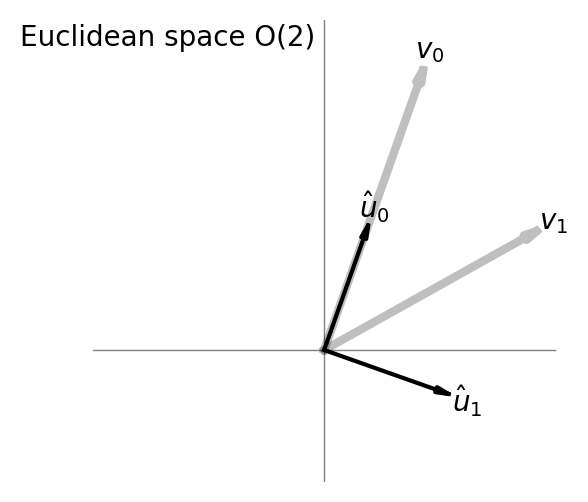
\includegraphics[width=0.33\textwidth]{E_v.png}%
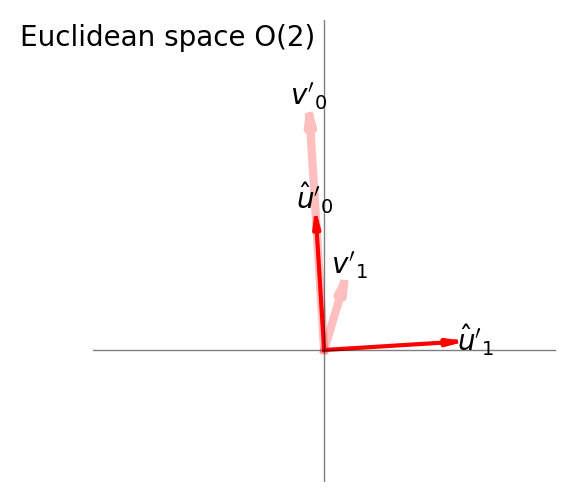
\includegraphics[width=0.33\textwidth]{E_vp.png}%
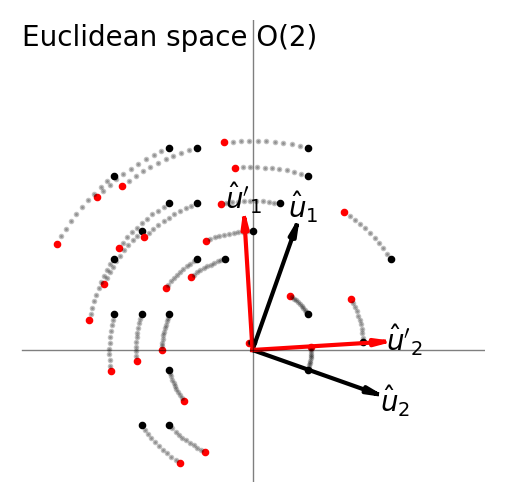
\includegraphics[width=0.33\textwidth]{E_Q.png}
\caption{A demonstration of orthogonalization and rotation in Euclidean 2-dimensional space O(2).
\textsl{Left:} Two vectors $v_1, v_2$ and the corresponding orthonormal vectors $\hat{u}_1, \hat{u}_2$ obtained by the orthogonalization procedure.
\textsl{Middle:} A different two vectors $v'_1, v'_2$ and the corresponding orthonormal vectors $\hat{u}'_1, \hat{u}'_2$.
\textsl{Right:} The action of the rotation operator $Q$ generated from the orthonomal pairs $\hat{u}_1, \hat{u}_2$ and $\hat{u}'_1, \hat{u}'_2$.
The black points rotate to the red points under the action of the operator $Q$.
The grey points in between are presented to guide the eye.\label{fig:Euclid}}
\end{figure}
The result of orthogonalization of two pairs of vectors in O(2) ($d=2$) is shown in \figref{fig:Euclid}.
Also shown in \figref{fig:Euclid} is the action of the rotation operator $Q$ derived from the basis vectors generated by those two orthogonalizations.

\section{Relativistic notation and transformations}\label{sec:notation}

There is a history of notation in special and general relativity.
Here we deliver a translation from traditional Einstein summation notation, and traditional language about boost, to a more linear-algebra-oriented notation.
After this Section, we will be using exclusively the linear-algebra notation, which is simpler (for us).

In Lorentz or Minkowski space, we think of there being a metric $\Lambda$ (often called $g_{\mu\nu}$), which is a $(d\plus1)\times(d\plus1)$ matrix that is \emph{not} positive definite.
The metric $\Lambda$ is diagonal with $+1$ in the first position and $-1$ repeated on all the remaining $d$ diagonal elements.
In $3\plus1$ this is
\begin{align}\label{eq:sig}
    \Lambda &= \begin{bmatrix}1 & 0 & 0 & 0\\
                              0 & -1 & 0 & 0\\
                              0 & 0 & -1 & 0\\
                              0 & 0 & 0 & -1\end{bmatrix} ~.
\end{align}
There is another possible signature---with $-1$ in the first position and $+1$ thereafter.
In this \documentname{} we choose the signature illustrated in \eqref{eq:sig}; nothing significant in our discussion changes if you choose the opposite signature.
Indeed, this is one of the main reasons to pursue the coordinate-free representations pursued here:
The coordinate-free representations don't care about the signature of your metric, or any other aspects of your coordinate system.\footnote{It is precisely because the choice of signature doesn't matter that physicists will constantly argue about it. We don't know many physicists who don't have a strong opinion about the signature.}

Given two vectors $u$, $v$ in $d\plus1$, old-school relativists tend to write the relativistic inner product $\inner{u}{v}\in\mathbb{R}$ (the scalar product or Minkowski inner product) as
\begin{align}
    \inner{u}{v} &= u^\mu\,v_\mu = v^\mu\,u_\mu ~,
\end{align}
where $\mu$ is a component index\footnote{In this \documentname{}, greek indexes like $\mu$, $\nu$ will be indexes over vector components (going from 1 to 4 in $3\plus1$, for example), and roman indexes like $i$, $j$ will be indexes over vectors or other things.} going from 1 to $d\plus1$, and the repeated index is (implicitly) summed.
The $u^\mu$ is a contravariant vector component and the $v_\mu$ is a covariant vector component.
Contravariant and covariant components are related as follows:
\begin{align}
    u^\mu &= \Lambda^{\mu\nu}\,u_\nu \equiv \sum_{\nu=1}^{d+1} \Lambda^{\mu\nu}\,u_\nu
    \\
    \inner{u}{v} &= u^\mu\,v_\mu = \Lambda^{\mu\nu}\,u_\mu\,v_\nu \equiv \sum_{\mu=1}^{d+1}\sum_{\nu=1}^{d+1} \Lambda^{\mu\nu}\,u_\mu\,v_\nu
\end{align}
where the $\Lambda^{\mu\nu}$ are the components of the metric $\Lambda$.
The implicit summations on the left of the ``$\equiv$'' signs are guided by the rules of what's called Einstein summation notation (\cite{summation}; it is a subset of the Ricci calculus~\cite{ricci}): Indexes can appear exactly once or exactly twice (and no more) and when they appear twice, one must be up and one must be down, and they are summed from 1 to $d+1$.
In quantum-mechanics (bra--ket) notation, a covariant vector is like a bra $\bra{v}$, and a contravariant vector is like a ket $\ket{v}$,
an inner product is a braket $\braket{u}{v}$, and an outer product (to appear below) is a ketbra $\ketbra{u}{v}$.

In linear algebra notation, if we think of $u$ and $v$ as being column vectors in $\mathbb{R}^{d+1}$ (or, to be extremely specific, $\mathbb{R}^{(d+1)\times 1}$), then we can write this same inner product as
\begin{align}\label{eq:inner}
    \inner{u}{v} &= u^\top\Lambda\,v ~.
\end{align}
We are going to use this notation going forward, not the Einstein summation notation.

In standard special-relativity lore, Lorentz transformations are taught as \emph{boost transformations} in which the assignment of the stationary observer is changed and the time and space axes change accordingly.
For our purposes, the Lorentz transformations also include spatial rotations, spatial reflections, and even time reflections (gasp!):
That is, for our purposes, an operator $Q$ is a valid Lorentz transformation if it is a member of the Lorentz group O($1,d$).
To be more specific, an operator $Q$ (which can be thought of as a $(d+1)\times(d+1)$ matrix) is a Lorentz transformation---is in O($1,d$)---if it preserves all inner products (scalar products). 
That is,
\begin{equation}
    Q \in \mbox{O($1,d$)} ~ \mbox{if and only if} ~ \inner{u}{v}=\inner{Q\,u}{Q\,v} ~ \mbox{for all $u,v$ in $\mathbb{R}^{d+1}$} ~ .\label{eq:lore1}
\end{equation}
This, in turn, will be true if and only if $Q$ leaves the metric unchanged:
\begin{equation}
    Q \in \mbox{O($1,d$)} ~ \mbox{if and only if} ~ Q^\top\Lambda\,Q=\Lambda ~ .\label{eq:lore2}
\end{equation}
This is our (surprising, perhaps) definition of the Lorentz transformation $Q$.
Note how similar the Lorentz-group statements \eqref{eq:lore1} and \eqref{eq:lore2} are to the orthogonal-group statements \eqref{eq:orth1} and \eqref{eq:orth2}.

For example, the simplest Lorentz space is O($1,1$) or $1\plus1$ ($d=1$).
In this case, the Lorentz transformations form a one-dimensional family; they are all of the form
\begin{align}
    Q &= \begin{bmatrix}\gamma & \beta\,\gamma \\ \beta\,\gamma & \gamma\end{bmatrix} ~\mbox{or}~
    \begin{bmatrix}-\gamma & -\beta\,\gamma \\ \beta\,\gamma & \gamma\end{bmatrix} ~\mbox{or}~
    \begin{bmatrix}\gamma & \beta\,\gamma \\ -\beta\,\gamma & -\gamma\end{bmatrix}  ~\mbox{or}~
    \begin{bmatrix}-\gamma & -\beta\,\gamma \\ -\beta\,\gamma & -\gamma\end{bmatrix} \label{eq:o11}
    \\
    \gamma &\equiv \frac{1}{\sqrt{1 - \beta^2}} \quad \text{and} \quad -1 < \beta < 1
\end{align}
In this simple case, $\beta$ is the dimensionless velocity of the boost, and $\gamma$ is the Lorentz factor.
The four choices in \eqref{eq:o11} correspond to even parity, reversing time (after the boost), reversing space (after the boost), and reversing both.\footnote{%
Many physicists would not permit reversals of time or space among the Lorentz transformations.
These reversals appear inevitably when we define the set of Lorentz transformations to be all the operators $Q$ such that $\Lambda=Q^\top\Lambda\,Q$, as we do.
So we depart here slightly from standard practice by being maximally inclusive.}
But in what follows we are going to develop \emph{coordinate-free forms} for the Lorentz transformations, in analogy to the coordinate-free forms for the rotation-reflection operators given in \secref{sec:od}.

Finally we remark that---because the metric is non-positive-definite---a nonzero vector $v$ in $d\plus1$ can come in three forms, \emph{timelike}, \emph{spacelike}, or \emph{lightlike} (sometimes \emph{null}):
\begin{align}
    v ~ \mbox{is timelike} &~ \mbox{if} ~ \inner{v}{v} > 0 \\
    v ~ \mbox{is lightlike} &~ \mbox{if} ~ \inner{v}{v} = 0 \\
    v ~ \mbox{is spacelike} &~ \mbox{if} ~ \inner{v}{v} < 0 ~.
\end{align}
(Technically, these definitions depend on the signature you chose for your metric; you would use the opposite language if you chose the opposite signature; see \secref{sec:notation}.)
Because Lorentz transformations $Q\in$~O($1,d$) preserve inner products, you can't Lorentz transform a vector from any one of these three categories to any other of these categories; the category is a Lorentz invariant property of the $(d\plus1)$-vector.

HOGG: ANALOGOUS to the Euclidean 2-d figure / diagram / example, make a Lorentz $1\plus1$ figure / diagram / example here.

\section{Relativistic orthogonalization}\label{sec:orth}

In Lorentz space we will still say that two vectors are ``orthogonal'' if their inner product is zero.
\begin{align}
    u,v ~\mbox{are orthogonal} ~ &\mbox{if and only if} ~ \inner{u}{v}=0 ~,
\end{align}
where the inner product is defined as in \eqref{eq:inner}.
This is great, but it leads to a strange consequence:
Any lightlike vector $v$ is \emph{orthogonal to itself}.
This is just one aspect of the oddness of orthogonality under the Lorentz metric:
It is also the case that orthogonal vectors aren't generally at 90 degrees with respect to each other; in fact angles aren't obviously defined for general vectors in spacetime.

We will still have linear dependence and independence exactly as in Euclidean space:
A set of $n\leq(d+1)$ vectors $v_j\in\mathbb{R}^{d+1}$ are linearly independent if there is no non-trivial set of amplitudes $a_j\in\mathbb{R}$ such that $\sum_{j=1}^n a_j\,v_j = 0$.

HOGG ASKS: DID we state the definition of linear independence above in the Euclidean part?

Now: How does orthogonalization and orthonormalization work in relativity?
Start with $n\leq d+1$ linearly independent vectors $v_1,v_2,\ldots,v_n$ in $\mathbb{R}^{d+1}$.
If these vectors are randomly generated, then with probability unity the straightforward generalization of Gram--Schmidt will work:
\begin{align}
    u_1 &\leftarrow v_1 \label{eq:rgs1}
    \\
    \mbox{then for each $j$ ($2\leq j\leq n$) in order:} ~~ u_j &\leftarrow v_j - \sum_{k=1}^{j-1} \frac{\inner{v_j}{u_k}}{\inner{u_k}{u_k}}\,u_k \label{eq:rgs2}
    \\
    \mbox{then for each $j$ ($1\leq j\leq n$):} ~~ \hat{u}_j &\leftarrow \frac{1}{\sqrt{|\inner{u_j}{u_j}|}}\,u_j ~, \label{eq:rgs3}
\end{align}
where we had to insert an absolute value inside the square-root operation because negative inner products will appear.
We're done. \emph{Ta-da!}
But we aren't really done, because the iteration step \eqref{eq:rgs2} involves dividing by an inner product, and inner products can vanish if the procedure accidentally produces a lightlike vector $u_j$ for some $j$.

In principle (and in practice if your context is adversarial), the orthogonalization procedure in \eqref{eq:rgs1} and \eqref{eq:rgs2} can produce a lightlike vector.
If you start with $n$ linearly independent vectors $v_j$, ($1\leq j\leq n$), begin the orthogonalization procedure, and then at some $j$ produce a lightlike $u_j$, here are the strategies:
\begin{enumerate}
    \item If all your input vectors $v_j$ are lightlike, then by construction, $u_1$ will be lightlike.
    Replace the first two input vectors $v_1, v_2$ with two (possibly randomly constructed) independent linear combinations of the $v_1$ and $v_2$.
    Re-start the orthogonalization.
    With high probability the orthogonalization will succeed.
    \item If not every one of your input vectors is lightlike, but the first one is, then by construction $u_1$ will be lightlike.
    Reorder the vectors such that the first vector is not lightlike and re-start the orthogonalization.
    With high probability the orthogonalization will succeed.
    \item If none of your input vectors is lightlike, but a lightlike $u_j$ is appearing, reorder the input vectors and re-start the orthogonalization.
    \item If all of the above fails, replace the $n$ input vectors $v_j$ with a randomly generated set of $n$ indepdent linear combinations of the original $n$ input vectors.
    With probability one, orthogonalization will succeed on this new set of inputs (and, by construction, it will span the same subspace as the original input vectors).
\end{enumerate}
These rules aren't extremely satisfying, because (unless you are extremely careful) they involve changing things like the orientation of the coordinate system.
We conjecture that there are better possible rules.

One comment to make is that orthogonalization is not necessarily numerically stable.
That is, a set of vectors can be formally linearly independent, but only barely (or not at all) at finite precision.
It is out of scope for us here, but there are methods to improve the stability of orthogonalizations (SOLE WHAT TO CITE?); these will be generalizable to the Lorentz space.

Another comment to make is that if you start with $n=d+1$ linearly independent vectors in $\mathbb{R}^{d+1}$, the outcome of the orthogonalization will be exactly one timelike vector and exactly $d$ spacelike vectors.
Importantly for what follows, \emph{the algorithm-generated set of normalized unit vectors $\hat{u}_1,\hat{u}_2,\ldots,\hat{u}_{d+1}$ will form a coordinate basis in spacetime}, with one timelike (time) axis vector and three orthogonal spacelike (spatial) axis vectors.

Now just like in O($d$) you can use the orthogonalization to make a subspace projection operator.
If you have $n$ $(d+1)$-vectors that span a subspace $\mathscr{T}$, then you can orthogonalize them and construct the subspace projection operator $\Pi_\mathscr{T}$
\begin{align}\label{eq:rproj}
    \Pi_\mathscr{T} &= \sum_{j=1}^n \frac{\hat{u}_j\,\hat{u}_j^\top\Lambda}{\inner{\hat{u}_j}{\hat{u}_j}} = \sum_{j=1}^n \frac{u_j\,u_j^\top\Lambda}{\inner{u_j}{u_j}} ~,
\end{align}
where the $\hat{u}_j$ are the orthogonal unit vectors, and the $u_j$ are the un-normalized orthogonal vectors; this differs from the result in \eqref{eq:oproj} in that we have to divide by an inner product $\inner{\hat{u}_j}{\hat{u}_j}$ to account for the sign of the inner product, and we have a right multiply of the metric $\Lambda$.
But notice that \eqref{eq:rproj} reduces to \eqref{eq:oproj} when the metric is the identity (and thus all inner products are positive.
This projection operator has the property that, for any vector $w\in\mathbb{R}^d$, the vector $\Pi_\mathscr{T}\,w$ will lie in the subspace $\mathscr{T}$ spanned by the $n$ original $(d\plus1)$-vectors $v_j$ that were orthogonalized.

If you have a full set of $n=d+1$ linearly independent vectors $v_j$, they will span the whole $(d\plus1)$-dimensional space, and the projection operator $\Pi_\mathscr{T}$ will become the identity $I_{d\plus1}$.
That is, if you have an orthonormal basis of $d+1$ unit vectors $\hat{u}_j$
\begin{align}
    I_{d\plus1} &= \sum_{j=1}^{d+1} \frac{\hat{u}_j\,\hat{u}_j^\top\Lambda}{\inner{\hat{u}_j}{\hat{u}_j}} = \sum_{j=1}^{d+1} \frac{u_j\,u_j^\top\Lambda}{\inner{u_j}{u_j}} ~,
\end{align}
where we have written it in terms of both the normalized and un-normalized orthogonal vectors; note that $\inner{\hat{u}_j}{\hat{u}_j}=\pm 1$.
In quantum-mechanical bra--ket notation, this expression for the identity becomes a standard formula in quantum mechanics:
\begin{align}
    I_{d\plus1} &= \sum_{j=1}^d \ketbra{\hat{u}_j}{\hat{u}_j}
    \\
    \ket{\hat{u}_j} &\equiv \hat{u}_j
    \\
    \bra{\hat{u}_j} &\equiv \frac{1}{\inner{\hat{u}_j}{\hat{u}_j}}\,\hat{u}_j^\top\Lambda ~,
\end{align}
where we have taken some liberties in defining the bra $\bra{\hat{u}_j}$, and we remind you that $\inner{\hat{u}_j}{\hat{u}_j}=\pm 1$.

Because the metric is its own inverse, if we right-multiply by the metric, we make a simple expression for the metric $\Lambda$ in terms of the basis vectors:
\begin{align}
    \Lambda &= \sum_{j=1}^{d+1} \frac{\hat{u}_j\,\hat{u}_j^\top}{\inner{\hat{u}_j}{\hat{u}_j}} = \sum_{j=1}^{d+1} \frac{u_j\,u_j^\top}{\inner{u_j}{u_j}} ~.
\end{align}
This expression is beautifully independent of the signature of the metric (mentioned in \secref{sec:notation}); it works for either signature.

\section{Vector-guided Lorentz transformations}\label{sec:lt}

HOGG ASKS: Have we clearly defined $d$-vectors and $(d\plus1)$-vectors?

All this work with unit vectors in special relativity is in the service of making coordinate-free expressions for arbitrary Lorentz transformations.
Consider two observers moving through spacetime.
One (unprime) is moving with $(d\plus1)$-velocity $u$ and the other (prime) is moving with $(d\plus1)$-velocity $u'$.
It is a property of any $(d\plus1)$-velocity that it is timelike, and that it has norm 1 (it is a unit vector), so we could have called these two $(d\plus1)$-velocities $\hat{u}$ and $\hat{u}'$.
Each of these two observers has a rest frame, and if $u-u'\neq 0$, those two reference frames are different.
What are the Lorentz transformations between the two reference frames?
That is, how do I construct transforms $Q\in$~O($1,d$) that boost $u$ to make it parallel to $u'$, and vice versa?

This problem looks similar to the problem in which we found rotations in O($d$) that align vectors in \secref{sec:od}.
We first perform two orthonormalizations, one for unprime and one for prime.
Then we build a Lorentz transformation operator $Q$ in much the same way as we built the rotation-reflection operator previously.

HOGG...FIRST write down the general LT in terms of unit vectors.
HOGG: Note that you have to match up the timelike and spacelike vectors.
HOGG: Note that you should probably start with a timelike vector.

HOGG...NOW Construct the particular LT we want from $p, p'$.

HOGG...MAYBE Show what you would have written in Einstein summation notation and in bra-ket notation.

\begin{figure}[t]
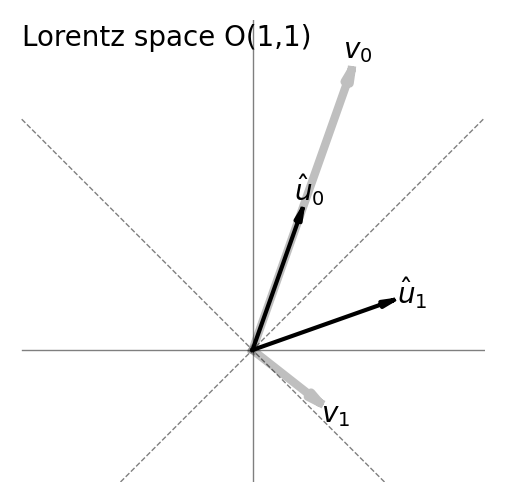
\includegraphics[width=0.33\textwidth]{L_v.png}%
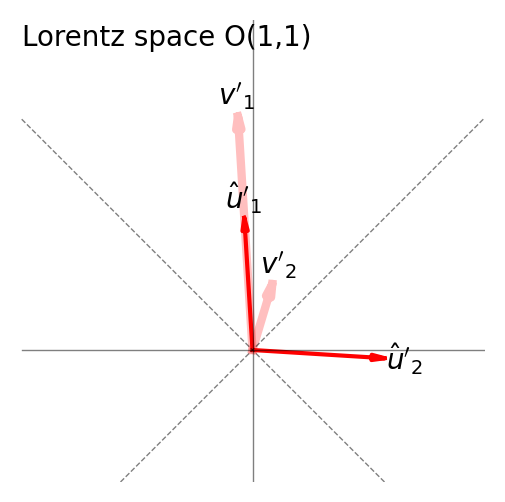
\includegraphics[width=0.33\textwidth]{L_vp.png}%
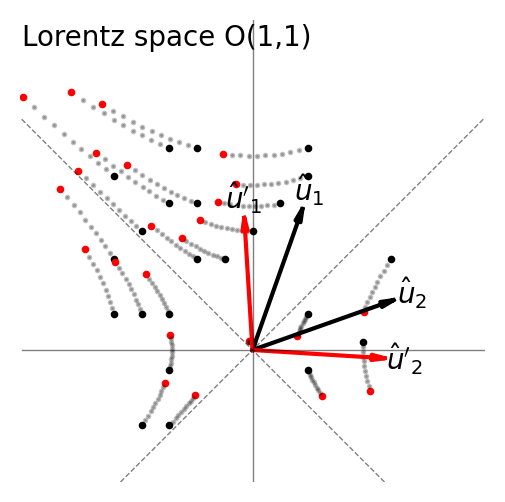
\includegraphics[width=0.33\textwidth]{L_Q.png}
\caption{A demonstration of orthogonalization and rotation in Lorentz $1\plus1$-dimensional space O(1,1).
The time coordinate (the first coordinate) is plotted on the vertical axis and the space coordinate (the second coordinate) is plotted on the horizontal axis.
\textsl{Left:} Two $(1\plus1)$-vectors $v_1, v_2$ and the corresponding orthonormal vectors $\hat{u}_1, \hat{u}_2$ obtained by the orthogonalization procedure.
Note that orthonormal vectors in $1\plus1$ neither look orthogonal nor normalized to the eye; the lightlike (null) lines are plotted to show that orthogonal $(1\plus1)$-vectors are reflected across null lines.
\textsl{Middle:} A different two $(1\plus1)$-vectors $v'_1, v'_2$ and the corresponding orthonormal vectors $\hat{u}'_1, \hat{u}'_2$.
\textsl{Right:} The action of the transformation operator (Lorentz transform) $Q$ generated from the orthonomal pairs $\hat{u}_1, \hat{u}_2$ and $\hat{u}'_1, \hat{u}'_2$.
The black points transform to the red points under the action of the operator $Q$.
The grey points in between are presented to guide the eye; 
note that they trace out not segments of circles (compare to \figref{fig:Euclid}) but instead segments of hyperbolae.\label{fig:Lorentz}}
\end{figure}
This is all demonstrated in \figref{fig:Lorentz}...

\section{Discussion}\label{sec:discussion}

HOGG: Much of this is very mathematical and theoretical.
However, the new parameterization of the Lorentz transformation in \secref{sec:lt} is useful and conceptually valuable.

HOGG: The hacks to fix the orthogonalization in \secref{sec:orth} are unsatisfying. Are there better solutions?

HOGG: Comment on numerical stability: This is an issue in general, but when $d\approx 3$, it isn't a big issue. See ``Modified Gram-Schmidt''.

SOLE: What can we say about spaces like O($2,9$), which might appear in string-like theories?
HOGG THINKS: Everything carries over to O($s,d$) for all $s,d$, although he SUSPECTS that some of the orthogonalization issues will get worse (numerically) as the dimensions $s,d$ get large.

All the code used to make the figures for this \documentname{} is available under an open-source license at HOGG: URL HERE.

\paragraph{Acknowledgements:}
It is a pleasure to thank
  Roger Blandford (Stanford), and
  Ben Blum-Smith (JHU)
for very valuable discussions.
This research was supported in part by XXX YYY.
The Flatiron Institute is a division of the Simons Foundation.

\raggedright
\printbibliography
\end{document}
